
写CMake时,有几个主要概念和语言特性需要知道。我们不会在这里详述语言的种种细节,若需要详细了解可以参考CMake的官方文档。下面的小节中,将简介主要概念和语言特性。后续章节将深入探讨其中细节。

完整文档地址\url{https://cmake.org/cmake/help/latest/manual/cmake-language.7.html}。

\subsubsubsection{1.6.1\hspace{0.2cm}CMake语言——鸟瞰全景}

CMake使用CMakeLists.txt文件的配置文件来确定构建规范。这些文件用脚本语言编写,通常也称为CMake。语言本身很简单,支持变量、字符串函数、宏、函数定义和导入其他CMake文件。

除了列表,不支持数据结构,如结构或类。但若操作得当,这种简单性使得CMake项目具有更好的可维护性。

语法基于关键字和以空格分隔的参数。例如,下面的指令会将相应的文件添加到库中:

\begin{lstlisting}[style=styleCMake]
target_sources(MyLibrary
                PUBLIC include/api.h
                PRIVATE src/internals.cpp src/foo.cpp)
\end{lstlisting}

PUBLIC和PRIVATE关键字表示文件链接到这个库时的可见性,并充当文件列表之间的分隔符。

此外,CMake语言支持“生成器表达式”,可以在生成构建系统时进行,通常用于为每个构建配置指定特殊信息。

\hspace*{\fill} \\ %插入空行
\noindent
\textbf{工程}

CMake会将各种构建工件(如库、可执行文件、测试和文档)组织到项目中。虽然不同项目可以相互封装,但这里需要一个根项目。每个CMakeLists.txt文件对应一个项目,所以每个项目必须在源目录中有一个单独的文件夹。

项目描述如下:

\begin{lstlisting}[style=styleCMake]
project(
  ch1_simple_executable
  VERSION 1.0
  DESCRIPTION "A simple C++ project to demonstrate basic CMake usage"
  LANGUAGES CXX
)
\end{lstlisting}

正在解析的当前项目存储在PROJECT\_NAME变量中。根项目存储在CMAKE\_PROJECT\_NAME中,这对于确定一个项目是独立的还是封装在另一个项目中很有用。从3.21版本开始,还有一个PROJECT\_IS\_TOP\_LEVEL变量来直接确定当前项目是否是顶层项目。此外,使用<PROJECT-NAME>\_IS\_TOP\_LEVEL,可以检测特定的项目是否为顶层项目。

下面是关于项目的其他内置变量,可以在根项目的值前加上CMAKE\_前缀。若没有在\texttt{project()}指令中定义,则字符串为空:

\begin{itemize}
\item 
PROJECT\_DESCRIPTION: 项目的描述字符串

\item 
PROJECT\_HOMEPAGE\_URL: 项目的URL字符串

\item 
PROJECT\_VERSION: 项目的完整版本信息

\item 
PROJECT\_VERSION\_MAJOR: 版本字符串的第一个数字

\item 
PROJECT\_VERSION\_MINOR: 版本字符串的第二个数字

\item 
PROJECT\_VERSION\_PATCH: 版本字符串的第三个数字

\item 
PROJECT\_VERSION\_TWEAK: 版本字符串的第四个数字
\end{itemize}

每个项目都有一个源目录和二进制目录,假设下面的例子中的每个CMakeLists.txt文件都定义了一个项目:

\begin{tcblisting}{commandshell={}}
.
├── CMakeLists.txt #defines project("CMakeBestPractices"...)
├── simple_executable
│      ├── CMakeLists.txt # defines project("Chapter 1"...)
\end{tcblisting}

当解析根目录下的CMakeLists.txt文件时,PROJECT\_NAME和CMAKE\_PROJECT\_NAME都将是CMakeBestPractices。当解析chapter01/CMakeLists.txt时,PROJECT\_NAME变量将变为“chapter1”,但CMAKE\_PROJECT\_NAME还是CMakeBestPractices,并设置在根文件夹中。

尽管项目可以嵌套,但最好以独立的方式编写。虽然它们可能依赖于文件层次结构中较低的其他项目,但应该没有必要将一个项目作为另一个项目的子项目的必要。可以在同一个CMakeLists.txt文件中使用多个\texttt{project()},但并不推荐这样做,其会使项目混乱,难以维护。通常,最好为每个项目创建一个CMakeLists.txt文件,并用子文件夹组织结构。

本书的GitHub库,包含了本书中的例子,以分层的方式组织,其中每一章都是一个单独的项目,可能包含更多的项目,用于不同的部分和示例。

虽然每个示例都可以单独构建,但也可以从库的根目录构建整本书的所有示例。

\hspace*{\fill} \\ %插入空行
\noindent
\textbf{变量}

变量是CMake语言的核心部分。可以使用\texttt{set}指令设置变量,使用\texttt{unset}指令删除变量。变量名区分大小写。下面的例子展示了如何设置一个名为MYVAR的变量,并将其赋值为1234:

\begin{lstlisting}[style=styleCMake]
set(MYVAR "1234")
\end{lstlisting}

要删除MYVAR变量,可以使用\texttt{unset}:

\begin{lstlisting}[style=styleCMake]
unset(MYVAR)
\end{lstlisting}

一般的代码约定使用全大写命名变量。在内部,变量总是表示为字符串。

这里,可以用\$符号和花括号来访问变量的值:

\begin{lstlisting}[style=styleCMake]
message(STATUS "The content of MYVAR are ${MYVAR}")
\end{lstlisting}

变量的引用可以嵌套,并由内而外求值:

\begin{lstlisting}[style=styleCMake]
${outer_${inner_variable}_variable}
\end{lstlisting}

变量的作用域可以通过以下方式确定:

\begin{itemize}
\item 
函数作用域:在函数内部设置的变量只在函数内部可见。

\item 
目录作用域:源树中的每个子目录绑定变量,并包括来自父目录的变量。

\item 
持久缓存:缓存的变量可以是系统的,也可以是用户定义的。在多次运行中保持它们的值不变。
\end{itemize}

将PARENT\_SCOPE选项传递给\texttt{set()}会使变量在父作用域中可见。

CMake提供了各种预定义变量,通常以CMAKE\_为前缀。完整的列表地址\url{https://cmake.org/cmake/help/latest/manual/cmake-variables.7.html}。

\hspace*{\fill} \\ %插入空行
\noindent
\textbf{列表}

尽管CMake在内部将变量存储为字符串,但可以在CMake中使用分号分隔值来处理列表。列表可以通过传递多个未加引号的变量给\texttt{set()},或直接作为一个分号分隔的字符串来创建:

\begin{lstlisting}[style=styleCMake]
set(MYLIST abc def ghi)
set(MYLIST "abc;def;ghi")
\end{lstlisting}

使用\texttt{list}指令可以通过修改列表内容、重新排序或查找内容来操作列表。下面的代码将在MYLIST中查询abc值的索引,然后检索该值并将其存储在名为ABC的变量中:

\begin{lstlisting}[style=styleCMake]
list(FIND MYLIST def ABC_INDEX) 
list(GET MYLIST ${ABC_INDEX} ABC)
\end{lstlisting}

要向列表追加一个值,可以使用APPEND 关键字。这里,xyz值会添加到MYLIST中:

\begin{lstlisting}[style=styleCMake]
list(APPEND MYLIST "xyz")
\end{lstlisting}

\hspace*{\fill} \\ %插入空行
\noindent
\textbf{缓存变量和选项}

CMake缓存了一些变量,以便后续的构建运行得更快,变量存储在CMakeCache.txt文件中。通常,不必手动编辑改文件,但对其修改可以用于调试构建。

所有用于配置构建的变量都会进行缓存。要缓存一个自定义变量ch1\_MYVAR,其值为foo值,可以使用\texttt{set}指令:

\begin{lstlisting}[style=styleCMake]
set(ch1_MYVAR foo CACHE STRING "Variable foo that configures bar")
\end{lstlisting}

注意,缓存变量必须有一个类型和一个文档字符串,以提供它们的快照。

大多数自动生成的缓存变量都标记为“高级”,这意味着它们在默认情况下对\texttt{cmake-gui}和\texttt{ccmake}中用户是隐藏的。要使它们可见,必须显式地切换。若有额外的缓存变量是由CMakeLists.txt文件生成的,也可以通过调用\texttt{mark\_as\_advanced(MYVAR)}指令来隐藏:

\begin{center}
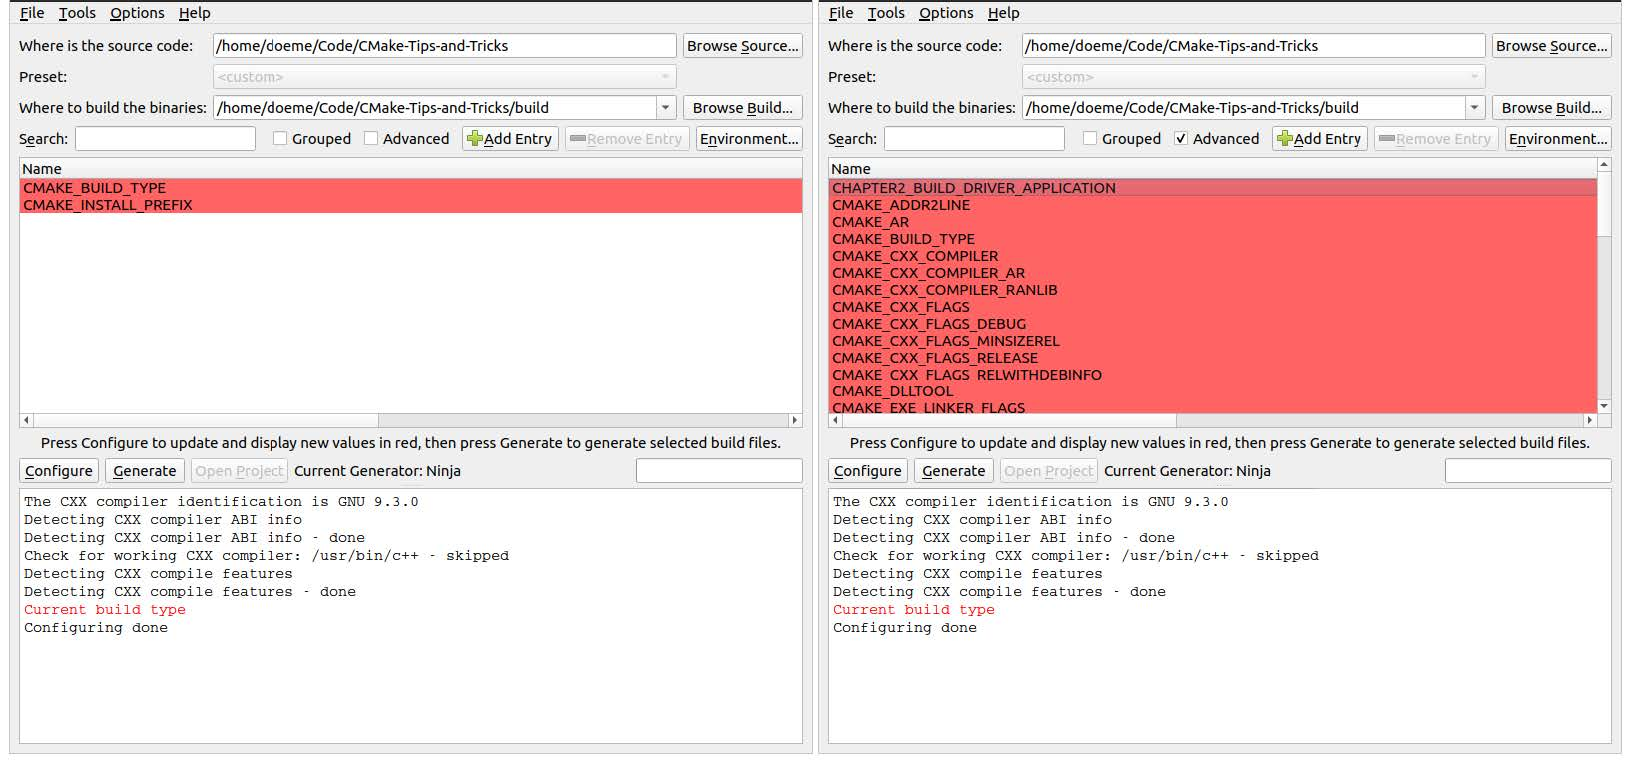
\includegraphics[width=0.8\textwidth]{content/1/chapter1/images/4.jpg}\\
图1.4  左边 —— \texttt{cmake-gui}没有显示标记为“高级”的变量。右边——标记“高级”复选框将显示所有标记为高级变量
\end{center}

根据经验,用户经常需要变更的选项或变量很少会标记为“高级”。

对于简单的布尔型缓存变量,CMake还提供了\texttt{option}指令,默认值为OFF,除非另有说明。也可以通过CMakeDependentOption模块相互依赖:

\begin{lstlisting}[style=styleCMake]
option(CHAPTER1_PRINT_LANGUAGE_EXAMPLES
	"Print examples for each language" OFF)

include(CMakeDependentOption)
cmake_dependent_option(CHAPTER1_PRINT_HELLO_WORLD
	"Print a nice greeting from chapter1" ON
	CHAPTER1_PRINT_LANGUAGE_EXAMPLES ON)
\end{lstlisting}

选项通常是指定简单项目配置的方法,是bool类型的缓存变量。若已经存在与该选项同名的变量,则\texttt{option}不会执行任何操作。

\hspace*{\fill} \\ %插入空行
\noindent
\textbf{属性}

CMake中的属性是附加到特定对象或CMake范围的值,如文件、目标、目录或测试用例。属性可以通过\texttt{set\_property}指令来设置。要读取属性的值,可以使用\texttt{get\_property}。默认情况下,\texttt{set\_property}会覆盖已经存储在属性中的值,可以通过传递\texttt{APPEND}或\texttt{APPEND\_STRING}将值添加到当前值中。

完整签名如下:

\begin{lstlisting}[style=styleCMake]
set_property(<Scope> <EntityName>
			[APPEND] [APPEND_STRING]
			PROPERTY <propertyName> [<values>])
\end{lstlisting}

作用域说明符可以有以下值:

\begin{itemize}
\item 
\texttt{GLOBAL}: 影响整个构建过程的全局属性。

\item 
\texttt{DIRECTORY <dir}>: 属性绑定到当前目录或<dir>中指定的目录,也可以直接使用\texttt{set\_directory\_properties}进行设置。

\item 
\texttt{TARGET <targets>}: 特定目标的属性,也可以使用\texttt{set\_target\_properties}进行设置。

\item 
\texttt{SOURCE <files>}: 将属性应用于源文件列表,也可以直接使用\texttt{set\_source\_files\_properties}进行设置。此外,还有\texttt{SOURCE DIRECTORY}和\texttt{SOURCE TARGET\_DIRECTORY}扩展选项:

\begin{itemize}
\item 
\texttt{DIRECTORY <dirs>}: 为目录范围内的源文件设置属性,该目录必须解析为当前目录或\texttt{add\_subdirectory}添加的目录。

\item 
\texttt{TARGET\_DIRECTORY <targets>}: 这将属性设置为创建指定目标的目录,目标必须在设置属性前已经存在。
\end{itemize}

\item 
\texttt{INSTALL <files>}: 这将设置已安装文件的属性,可以用来控制\texttt{cpack}的行为。

\item 
\texttt{TEST <tests>}: 这将设置测试的属性,也可以直接使用\texttt{set\_test\_properties}进行设置。

\item 
\texttt{CACHE <entry>}: 这将设置缓存变量的属性。最常见的方法包括将变量设置为高级或向其添加文档字符串。
\end{itemize}

支持的属性的完整列表,请查阅\url{https://cmake.org/cmake/help/latest/manual/cmakeproperties.7.html}。

当修改属性时,可以使用\texttt{set\_target\_properties}和\texttt{set\ test\_properties},而非\texttt{set\_property}。使用显式指令可以避免属性名之间的错误和混淆,可读性会更强。还有一个\texttt{define\_property}指令,其会创建一个不设置值的属性。我们不建议使用,因为属性总需要有一个默认值。

\hspace*{\fill} \\ %插入空行
\noindent
\textbf{循环和条件}

和其他编程语言一样,CMake支持条件块和循环块。条件块位于\texttt{if()}、\texttt{elseif()}、\texttt{else()}和\texttt{endif()}语句之间。条件使用各种关键字表示。

一元关键字可以在值前加前缀:

\begin{lstlisting}[style=styleCMake]
if(DEFINED MY_VAR)
\end{lstlisting}

条件中使用的一元关键字如下:

\begin{itemize}
\item 
\texttt{COMMAND}: 若提供的值是命令,则为True

\item 
\texttt{EXISTS}: 检查文件或路径是否存在

\item 
\texttt{DEFINED}: 若值是一个已定义的变量,则为True
\end{itemize}

此外,还有一元文件系统的条件:

\begin{itemize}
\item 
\texttt{EXISTS}: 若给定的文件或目录存在,则为True

\item 
\texttt{IS\_DIRECTORY}: 检查提供的路径是否为目录

\item 
\texttt{IS\_SYMLINK}: 若提供的路径是符号链接,则为True

\item 
\texttt{IS\_ABSOULTE}: 检查提供的路径是否为绝对路径
\end{itemize}

二元测试比较两个值,并放在要比较的值之间:

\begin{lstlisting}[style=styleCMake]
if(MYVAR STREQUAL "FOO")
\end{lstlisting}

二元运算符如下:

\begin{itemize}
\item 
\texttt{LESS},\texttt{GREATER},\texttt{EQUAL},\texttt{LESS\_EQUAL}和\texttt{GREATER\_EQUAL}: 比较数值。

\item 
\texttt{STRLESS},\texttt{STREQUAL},\texttt{STRGREATER},\texttt{STRLESS\_EQUAL}和\texttt{STRGREATER\_EQUAL}: 按字典序比较字符串。

\item 
\texttt{VERSION\_LESS},\texttt{VERSION\_EQUAL},\texttt{VERSION\_GREATER},\texttt{VERSION\_LESS\_EQUAL}和\texttt{VERSION\_GREATER\_EQUAL}: 比较版本字符串。

\item 
\texttt{MATCHES}: 使用正则表达式进行匹配。

\item 
\texttt{IS\_NEWER\_THAN}: 比较两个文件中哪一个最近修改过。但这不是很精确,若两个文件具有相同的时间戳,也会返回True。还有更令人困惑的结果,若其中任何一个文件丢失,结果也为True。
\end{itemize}

最后,就是布尔运算符\texttt{OR}、\texttt{AND}和\texttt{NOT}。

循环可以通过\texttt{while()}和\texttt{endwhile()},或\texttt{foreach()}和\texttt{endforeach()}实现。循环可以使用\texttt{break()}终止,\texttt{Continue()}会中止当前的迭代并立即开始下一个迭代。

while循环接受与if语句相同的条件。下面的示例只要MYVAR小于5就会循环。为了增加变量,我们使用\texttt{math()}指令:

\begin{lstlisting}[style=styleCMake]
set(MYVAR 0)
while(MYVAR LESS "5")
	message(STATUS "Chapter1: MYVAR is '${MYVAR}'")
	math(EXPR MYVAR "${MYVAR}+1")
endwhile()
\end{lstlisting}

除了while循环之外,CMake还知道用于遍历列表或范围的循环:

\begin{lstlisting}[style=styleCMake]
foreach(ITEM IN LISTS MYLIST)
# do something with ${ITEM}
endforeach()
\end{lstlisting}

for循环可以使用\texttt{RANGE}关键字:

\begin{lstlisting}[style=styleCMake]
foreach(ITEM RANGE 0 5)
# do something with ${ITEM}
endforeach()
\end{lstlisting}

\texttt{foreach()}的\texttt{RANGE}版本可以只用一个结束值,不过指定开始值和结束值是一个很好的习惯。

\hspace*{\fill} \\ %插入空行
\noindent
\textbf{函数}

函数由\texttt{function()}/\texttt{endfunction()}定义。函数为变量创建了一个新的作用域,因此所有在内部定义的变量都不能从外部访问,除非将\texttt{PARENT\_SCOPE}选项传递给\texttt{set()}。

函数不区分大小写,通过\texttt{function}后的名称加上圆括号来使用函数:

\begin{lstlisting}[style=styleCMake]
function(foo ARG1)
# do something
endfunction()
# invoke foo with parameter bar
foo("bar")
\end{lstlisting}

函数是使CMake部分可重用方法,当在做大型项目时,函数会经常使用。

\hspace*{\fill} \\ %插入空行
\noindent
\textbf{宏}

CMake宏使用\texttt{macro()}/\texttt{endmacro()}定义,有点像函数。不同的是,函数参数是真变量,而在宏中是字符串替换。这意味着必须使用大括号访问宏的所有参数。

另一个区别是,通过调用函数,作用区域转移到函数内部。执行宏时,就好像宏的主体粘贴到调用位置一样,宏不会创建变量和控制流的作用域。因此,避免在宏中调用\texttt{return()}。

\hspace*{\fill} \\ %插入空行
\noindent
\textbf{目标}

CMake的构建系统会组织一组逻辑目标,这些逻辑目标对应于可执行文件、库或自定义命令或工件,如文档或类似的文件。

CMake中有三种主要的方法来创建目标——\texttt{add\_executable},\texttt{add\_library}和\texttt{add\_custom\_target}。前两个用于创建可执行文件和静态或动态库,而第三个可以包含要执行的定制命令。

目标间可以相互依赖,因此一个目标必须在另一个目标之前建立。

在为构建配置或编译器选项设置属性时,使用目标变量是个好习惯。一些目标属性具有可见性修饰符,如\texttt{PRIVATE}、\texttt{PUBLIC}或\texttt{INTERFACE},以表示哪些需求是可传递的——哪些属性必须由依赖的目标“继承”。


\hspace*{\fill} \\ %插入空行
\noindent
\textbf{生成器表达式}

生成器表达式是在构建的配置阶段进行的语句。大多数函数允许使用生成器表达式,只有少数例外。以\texttt{\$<OPERATOR:VALUE>}的形式使用,其中\texttt{OPERATOR}或直接使用,或与VALUE进行比较。这里,可以将生成器表达式看作小型的内联if语句。

下面的例子中,若编译器是GCC、Clang或Apple Clang,则使用生成器表达式为my\_target启用\texttt{-Wall}编译器标志。注意GCC的\texttt{COMPILER\_ID}标识为"GNU":

\begin{lstlisting}[style=styleCMake]
target_compile_options(my_target PRIVATE
	"$<$<CXX_COMPILER_ID:GNU,Clang,AppleClang>:-Wall>")
\end{lstlisting}

若\texttt{CXX\_COMPILER\_ID}变量匹配GNU, Clang, AppleClang列表中任意一个,则附加\texttt{-Wall}选项到目标——也就是my\_target。生成器表达式在编写独立于平台和编译器的CMake文件时非常方便。

除了查询值,生成器表达式还可以用于转换字符串和列表:

\begin{lstlisting}[style=styleCMake]
$<LOWER_CASE:CMake>
\end{lstlisting}

这将输出“cmake”。

想要了解生成器表达式更多详情,可参阅\url{https://cmake.org/cmake/
help/latest/manual/cmake-generator-expressions.7.html}。

CMake支持各种构建系统、编译器和链接器,所以经常用于为不同的平台构建软件。下一节中,将学习如何在CMake中使用不同的工具链,以及如何配置不同的构建类型,如Debug或Release。

\hspace*{\fill} \\ %插入空行
\noindent
\textbf{CMake策略}

对于顶层的CMakeLists.txt文件的第一行,必须要有\texttt{cmake\_minimum\_required},因为其会设置用于构建项目的内部CMake策略。

策略用于保持跨多个CMake版本的向后兼容性,可以配置为使用OLD行为,所以CMake的行为需要向后兼容,或者配置为NEW,使新策略生效。由于每个新版本都将引入新的规则和功能,因此将使用策略来警告向后兼容性问题。可以使用\texttt{cmake\_policy}禁用或启用策略。

下面的例子中,\texttt{CMP0121}策略设置为向后兼容的值。\texttt{CMP0121}在CMake 3.21引入,用于检查\texttt{list()}的索引变量是否为有效格式——是否为整数:

\begin{lstlisting}[style=styleCMake]
cmake_minimum_required(VERSION 3.21)
cmake_policy(SET CMP0121 OLD)

list(APPEND MYLIST "abc;def;ghi")
list(GET MYLIST "any" OUT_VAR)
\end{lstlisting}

通过设置\texttt{cmake\_policy(SET CMP0121 OLD)},启用向后兼容,并且前面的代码不会产生警告,尽管这里使用“any”(不是一个整数)索引访问MYLIST。

在配置步骤中将策略设置为NEW将会抛出一个错误——\texttt{[build] list index: any is not a valid index}。

\begin{tcolorbox}[colback=blue!5!white,colframe=blue!75!black,title=除非包含遗留项目,否则避免设置策略]
通常,策略应该通过\texttt{cmake\_minimum\_required}来控制,而不是通过更改单个策略来控制。更改策略常用于,将历史遗留项目作为子文件夹包含在其中时。
\end{tcolorbox}

我们已经了解了用于配置构建系统的CMake语言背后的基本概念,CMake用于为不同类型的构建和语言生成构建指令。下一节中,我们将了解如何指定要使用的编译器,以及如何配置构建。












